% -*- root: cuthesis_masters.tex -*-

%In this chapter we present related work on ...

Software systems are expected to serve millions of concurrent requests~\cite{arlitt2000workload}. However, the systems are first tested to ensure that they are working correctly under a certain load(s). This load is also known as the rate at which the system is processing the requests. 
In this chapter, we discuss the motivation behind our work and similar studies in the field of performance engineering. We later survey the state-of-the-art literature that is related to our work.

\section{Background}

Generally, performance assurance activities are carried out by analyzing the system responses on a variety of workloads. For example, to detect performance issues, the system performance is analyzed after applying a workload. This workload profile depicts the normal workload of the system once it is functional in the field~\cite{464549}.


\subsection{Performance Testing}

Although there may be some similarities present between performance and load testing, performance testing is mainly focused to detect primarily performance related performance with the software system. For example, response time, throughput and resource utilization.~\cite{Barna:2011,6032540,Gorton}

Performance test is detailed than load testing as it may be used to cover designs ~\cite{csurgay1999performance,denaro2004early,denaro2005performance}, algorithms ~\cite{cangussu2009segment,cangussu2007reducing}, and system configurations ~\cite{hoskins2005software,pozin2011models,sopitkamol2005method}. The goal behind performance testing may be to test performance requirements~\cite{pozin2011models} or exploratory. For example, to answer questions such as how do various configurations impact the performance of the system ~\cite{Menasce:2000,Menasce:1994,Menasce:2001,pozin2011models}.

\subsubsection{What is a test execution?}



Before the phase of text execution, practitioners have to develop the test for the system. It is based on either the realistic usage of the system when functional or with the goal to uncover problems \cite{jiang2015survey}.
Once the test is developed, it is followed by its execution. 

\begin{figure*}[thb!]
	\centering
	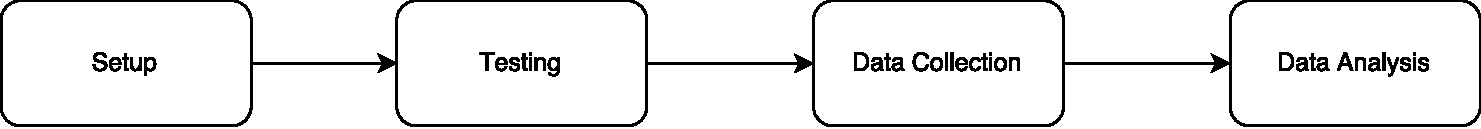
\includegraphics[width=1\textwidth]{figures/bck1.pdf}
	\caption{Test execution phases}
	\label{fig:test_phases}
\end{figure*}

As shown in figure \ref{fig:test_phases}, the lifecycle of a typical performance test is made up of four phases. 

\subsubsection{Setup and Testing}

~\textit{Setup}, that is system and test execution setup. ~\textit{Testing}, that is the actual phase where the test is run and terminated at the end of the time frame. ~\textit{Data Collection}, that is the phase where the performance metrics and executions logs are collected and further analyzed in the fourth phase \cite{jiang2015survey}.

The term~\textit{setup} is further divided into two sub-terms. The setup for the system and the setup for the text execution system. The former deals with making sure that the system or~\textit{SUT} is operational and fully functional. This may also include setting up servers and other functionalities attached to the system for example, database servers. The latter engulfs configuring and using the load test drivers (for example, WebLoad~\cite{webload}, HP LoadRunner~\cite{loadrunner}, Apache Jmeter ~\cite{apachejmeter}) in addition to setting up the testing environment. In order to record the performance metrics, performance monitoring tools are set up, e.g. Perfmon~\cite{perfmon}, Psutil~\cite{psutil}, etc. 

Following the setup, the system is tested by applying load. The results are concurrently recorded. Practitioners may terminate the load based on the following techniques:

\begin{itemize}
	\item Continuous: Testing until it is topped manually by practitioners~\cite{4017687}.
	\item Timer-Based: The test runs for a specific duration of time~\cite{4017687}.
	\item Counter-Based: The load is stopped after a certain number of requests sent or received~\cite{4017687}.
	\item Statistic-Based: A comparatively newer technique where the metric of interest is captures till it is statistically stable. This serves a high confidence level when analyzing the metric~\cite{mansharamani2010performance,snellman2011towards}.
\end{itemize}

\subsubsection{Data and Metrics Collection}

During the course of loading the system and running the tests, the data is monitored and recored. The data collected is in the form of logs and performance metrics. These performance metrics may be higher-level (e.g. throughput, response time, etc.) or lower-level (e.g. CPU utilization, memory usage, etc.) It is necessary that the monitoring or recording tool does not induce extra overhead on the system. This may lead to biased results~\cite{mytkowicz2010evaluating}.

\subsubsection{Data Analysis}
We discuss in detail the approaches to analyze data in section \ref{sec:related}.


\subsection{What are the differences between load testing, stress testing and performance testing?}

Although there are similarities between with these three types of testing techniques, for example all of these are carried out after functional testing, we now differentiate between the application of these tests.

\subsubsection{Load Testing}

The rate at which which the requests are submitted to a system is called the load~\cite{Beizer:1984}. This system is more commonly known as system under test or~\textit{SUT}. Load testing is carried out later than conventional testing in a software's life. This may be done on a prototype or a working system than a design or a model. Load testing is used to detect load related problems. For example, deadlocks, buffer overflows, high response times and low throughput~\cite{464549,Barna:2011,6032540}. 

In some exceptional cases where the non-functional requirements are not present, one of ways to determine if the test has passed is by comparing it to the results of the previous version. This is also known as the "no-worse-than-before" principle. As the name suggests, the version being tested should be, if not better, equal to the previous version.~\cite{Dumke:2001}

\subsubsection{Stress Testing}

Stress testing is testing the application under "stress" or extreme load. This can be used to detect how resilient the system or to detect further load-related problems. For example, memory leaks and deadlocks. These "stressful" conditions for the system can be either load related(normal ~\cite{zhang2002automated,kalita2011investigation,chakravarty2010stress} or heavy load ~\cite{Dillenseger2009,kalita2011investigation,huebner2001performance}) or limited resources allocated/failures (for example, disk or database failures) ~\cite{acharya2009mining}. We noted that in some cases it may also be used to detect the competency of the SUT \cite{garousi2010genetic,garousi2008empirical,garousi2006traffic,garousi2008traffic}.


Having stated all of the above, there are instances where the interest of a performance test may overlap with load testing pr stress testing and vice-versa. For example, to check robustness of the system when put in extreme conditions, or to check how an algorithm works when handling large files. We observe that the terms performance testing~\cite{Dillenseger2009,Menasce02loadtesting,Menasce:2002}, load testing ~\cite{536461,Bayan:2008,perf_load_stress,perf_web} and stress testing~\cite{Bayan:2008,Yang:1996,4020172} are also used interchangeably. 

We focus on performance testing, which is to detect performance related behavior of our~\textit{SUT}.


\section{Literature Review}
\label{sec:related}
In this section, we discuss the motivation and related work of this thesis in broadly three subsections: 1) analyzing performance metrics from performance testing, 2) analysis of VM overhead and 3) performance testing and bug detection.


\subsection{Analyzing performance testing results} 

Prior research has proposed a slew of techniques to analyze performance testing results, i.e. performance metrics. Such techniques typically examine three different aspects of the metrics: 1) single performance metric, 2) the relationship between performance metrics, and 3) statistical modeling based on performance metrics.


\subsubsection{Single performance metric}
\label{sec:relatedindividual}
Nguyen \textit{et al$.$}~\cite{Nguyen:2012:ADP:2188286.2188344} introduce the concept of using control charts~\cite{shewhart1931economic} in order to detect performance regressions. Control charts use a predefined threshold to detect performance anomalies. However control charts assume that the output follows a uni-model distribution, which may be an inappropriate assumption for performance. Nguyen \textit{ et al$.$} propose an approach to normalize performance metrics between heterogeneous environments and workloads in order to build robust control charts. %However, the experiments are only carried out on the virtual machines in contrast to our approach.

Malik \emph{et al$.$}~\cite{Malik:2010:ACL:1955601.1955936, haroon} propose approaches that cluster performance metrics using Principal Component Analysis (PCA). Each component generated by PCA is mapped to performance metrics by a weight value. The weight value measures how much a metric contributes to the component. For every performance metric, a comparison is performed on the weight value of each component to detect performance regressions.

Heger \emph{et al$.$}~\cite{DBLP:conf/wosp/HegerHF13} present an approach that uses software development history and unit tests to diagnose the root cause of performance regressions. In the first step of their approach, they leverage Analysis of Variance (ANOVA) to compare the response time of the system to detect performance regressions. Similarly, Jiang \emph{et al$.$}~\cite{jackicsm2009} extract response time from system logs. Instead of conducting statistical tests, Jiang \emph{et al$.$} visualize the trend of response time during performance tests, in order to identify performance issues.


\subsubsection{Relationship between performance metrics}
\label{sec:relatedrelation}

Malik \emph{et al$.$}~\cite{5635038} leverage Spearman's rank correlation to capture the relationship between performance metrics. The deviance of correlation is calculated in order to pinpoint which subsystem should take responsibility of the performance deviation.

Foo \emph{ et al$.$}~\cite{foo2010mining} propose an approach that leverages association rules in order to address the limitations of manually detecting performance regressions in large scale software systems. Association rules capture the historical relationship among performance metrics and generate rules based on the results of prior performance tests. Deviations in the association rules are considered signs of performance regressions.

Jiang \emph{et al$.$}~\cite{5270324} use normalized mutual information as a similarity measure to cluster correlated performance metrics. Since metrics in one cluster are highly correlated, the uncertainty among metrics in the cluster should be low. Jiang \emph{et al$.$} leverage entropy from information theory to monitor the uncertainty of each cluster. A significant change in the entropy is considered as a sign of a performance fault. 


\subsubsection{Statistical modeling based on performance metrics}
\label{sec:relatedmodel}

Xiong \textit{et al$.$}~\cite{xiong2013vperfguard} proposed a model-driven approach named \textit{vPerfGuard} to detect software performance regressions in a cloud-environment. The approach builds models between workload metrics and a performance metric, such as CPU. The models can be used to detect workload changes and assists in identifying performance bottlenecks. Since the usage of \emph{vPerfGuard} is typically in a virtual environment, our study may help the future evaluation of \textit{vPerfGuard}. Similarly, Shang \textit{ et al.}~\cite{Shang:2015:ADP:2668930.2688052} propose an approach of including only a limited number of performance metrics for building statistical models. The approach leverages an automatic clustering technique in order to find the number of models to be build for the performance testing results. By building statistical models for each cluster, their approach is applicable to detect injected performance regressions. 

Cohen \textit{et al$.$}~\cite{cohen2004correlating} propose an approach that builds probabilistic models, such as Tree-Augmented Bayesian Networks, to examine the causes that target the changes in the system's response time. Cohen \textit{et al$.$}~\cite{Cohen:2005:CIC:1095810.1095821} also proposed that system faults can be detected by building statistical models based on performance metrics. The approaches of Cohen \textit{et al$.$}~\cite{cohen2004correlating, Cohen:2005:CIC:1095810.1095821} were improved by Bodik \textit{et al.}~\cite{bodik2008hilighter} by using logistic regression models.

Jiang \emph{et al$.$}~\cite{Jiang:2009:SMM:1555228.1555233} propose an approach that improves the Ordinary Least Squares regression models that are built from performance metrics and use the model to detect faults in a system. The authors conclude that their approach is more efficient in successfully detecting the injected faults than the current linear-model approach.

On one hand, none of the prior research discusses the impact of their approaches results in virtual and physical environments, which motivates the empirical study that is conducted in this thesis. On the other hand, since there are hardly two identical performance testing results, we do no compare the raw data of performance testing results from virtual and physical environments. Instead, we conduct our case study in the context of all the above three types of analyses, in order to see the impact when practitioners use such analyses on performance testing results. Our findings can help better evaluate and understand the findings from the aforementioned research. 



\subsection{Analysis of VM overhead}

Kraft \textit{et al$.$}~\cite{kraft2011io} discuss the issues related to disk I/O in a virtual environment. They examine the performance degradation of disk request response time by recommending a trace-driven approach. Kraft \textit{et al.} emphasize on the latencies existing in virtual machine requests for disc IO due to increments in time associated with request queues. 

Aravind \textit{et al$.$}~\cite{menon2005diagnosing} audit the performance overhead in Xen virtual machines. They uncover the origins of overhead that might exist in the network I/O causing a peculiar system behavior. However, there study is limited to Xen virtual machine only while mainly focusing on network related performance overhead.

Brosig \textit{et al$.$}~\cite{brosig2013evaluating} predict the performance overhead of virtualized environments using Petri-nets in Xen server. The authors focused on the visualization overhead with respect to queuing networks only. The authors were able to accurately predict server utilization but had significant errors for multiple VMs.


Huber \textit{et al$.$}~\cite{huber2011evaluating} present a study on cloud-like environments. The authors compare the performance of virtual environments and study the degradation between the two environments. Huber \textit{et al$.$} further categorize factors that influence the overhead and use regression based models to evaluate the overhead. However, the modeling only considers CPU and memory.


Luo \textit{et al$.$}~\cite{Luo:2016:MPR:2901739.2901765} converge the set of inputs that may cause software regression. They apply genetic algorithms to detect such combinations. Netto \textit{et al$.$} \cite{netto2011evaluating} present a similar study to compare performance metrics generated via load tests between the two environments. However, the author did not analyse the results from a statistical perspective.

Prior research focused on the overhead of virtual environments without considering the impact of such overhead on performance testing and assurance activities. In this thesis, we evaluate the discrepancy between virtual and physical environments by focusing on the impact of performance testing results analyses and investigate whether such impact can be reduced in practice.


\subsection{Performance testing and bug detection}

There exists much research on performance testing and bug detection. Nistor \textit{et al$.$}~\cite{Nistor} detect the presence of functional and loop-related performance bugs with the help of their developed tool. Jin \textit{et al$.$} \cite{Jin} present a study on a wide range of performance bugs. The authors examined real-world performance bugs and developed rule-based performance bug detection tools. Nistor \textit{et al$.$}~\cite{nistor_2} in another study highlight that automated tool based performance bug detection is limited. The authors also comment that performance bugs are mostly detected by code reasoning rather than seeing the effects of the system by the end users. Tsakiltsidis \textit{et al$.$}~\cite{Tsakiltsidis} use prediction models to detect and predict performance bugs based on extraction from source code repositories. Malik \textit{et al$.$}~\cite{h_malik_p_bugs} present a study to uncover functional bugs via load testing. The authors propose an approach to reduce the large amount of performance metrics at the end of a load test by principal component analysis. Zaman \textit{et al$.$}~\cite{zaman_p_bugs} study the tracking and fixing of performance bugs.

However, none of the above mentioned performance bug detection approach has been applied in different environments. In most of the cases, the environment is not explicitly mentioned. Hence, to generalize the findings across environments remains an open topic.
